\RequirePackage{luatex85}
\documentclass[amsmath]{article}
\usepackage{amsmath}
\usepackage{amssymb}
\usepackage{geometry,contour}
\usepackage{tikz}
\usetikzlibrary{positioning}
\usetikzlibrary{decorations.text}
\usetikzlibrary{decorations.pathmorphing}
\usetikzlibrary{decorations.text}
\usetikzlibrary{decorations.pathmorphing}
\definecolor{darkolivegreen}{rgb}{0.3, 0.5, 0.2}
\geometry{legalpaper, landscape, margin=0.0in}
\paperheight 2.5in
\paperwidth 5.5in


\begin{document}
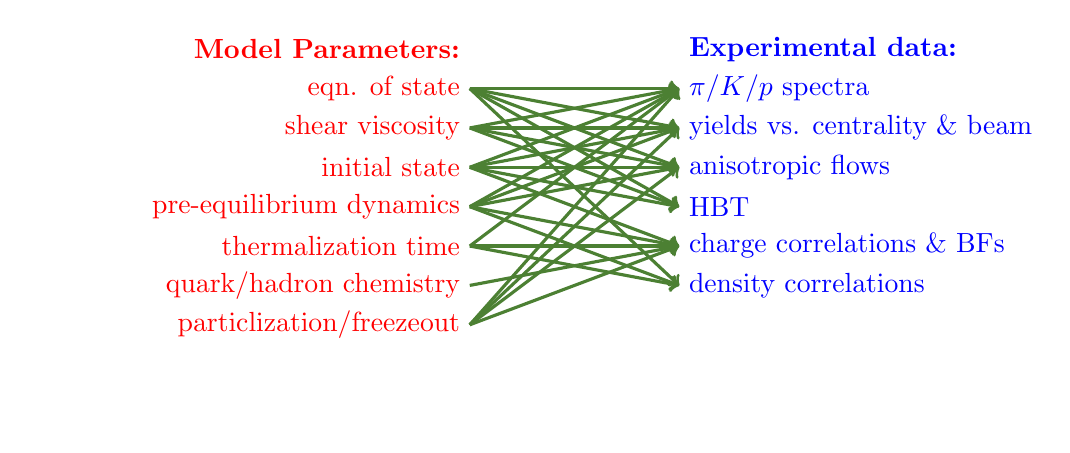
\begin{tikzpicture}
\node(a)[align=right] at (0,0) {\color{red} \bf Model Parameters:};
\node(b)[below=of a.east,anchor=east, yshift=.5cm] {\color{red} eqn. of state};
\node(c)[below=of b.east,anchor=east, yshift=.5cm] {\color{red} shear viscosity};
\node(d)[below=of c.east,anchor=east, yshift=.5cm] {\color{red} initial state};
\node(e)[below=of d.east,anchor=east, yshift=.5cm] {\color{red} pre-equilibrium dynamics};
\node(f)[below=of e.east,anchor=east, yshift=.5cm] {\color{red} thermalization time};
\node(g)[below=of f.east,anchor=east, yshift=.5cm] {\color{red} quark/hadron chemistry};
\node(h)[below=of g.east,anchor=east, yshift=.5cm] {\color{red} particlization/freezeout};

\node(A) at (6.3,0) {\color{blue} \bf Experimental data:};
\node(B) [below=of A.west,anchor=west, yshift=.5cm] {\color{blue} $\pi$/$K$/$p$ spectra};
\node(C) [below=of B.west,anchor=west, yshift=.5cm] {\color{blue} yields vs. centrality \& beam};
\node(D) [below=of C.west,anchor=west, yshift=.5cm] {\color{blue} anisotropic flows};
\node(E) [below=of D.west,anchor=west, yshift=.5cm] {\color{blue} HBT};
\node(F) [below=of E.west,anchor=west, yshift=.5cm] {\color{blue} charge correlations \& BFs};
\node(G) [below=of F.west,anchor=west, yshift=.5cm] {\color{blue} density correlations};

\node(bh)[below=of g.east,anchor=east, yshift=-.5cm] {\phantom{\color{red} Transver Momentum Broadening $\hat{q}$}};

\draw[->, color=darkolivegreen,line width=.4mm] (b.east)--(B.west);
\draw[->, color=darkolivegreen,line width=.4mm] (b.east)--(C.west);
\draw[->, color=darkolivegreen,line width=.4mm] (b.east)--(D.west);
\draw[->, color=darkolivegreen,line width=.4mm] (b.east)--(E.west);
\draw[->, color=darkolivegreen,line width=.4mm] (b.east)--(G.west);

\draw[->, color=darkolivegreen,line width=.4mm] (c.east)--(B.west);
\draw[->, color=darkolivegreen,line width=.4mm] (c.east)--(C.west);
\draw[->, color=darkolivegreen,line width=.4mm] (c.east)--(D.west);
\draw[->, color=darkolivegreen,line width=.4mm] (c.east)--(E.west);


\draw[->, color=darkolivegreen,line width=.4mm] (d.east)--(B.west);
\draw[->, color=darkolivegreen,line width=.4mm] (d.east)--(C.west);
\draw[->, color=darkolivegreen,line width=.4mm] (d.east)--(D.west);
\draw[->, color=darkolivegreen,line width=.4mm] (d.east)--(E.west);
\draw[->, color=darkolivegreen,line width=.4mm] (d.east)--(F.west);

\draw[->, color=darkolivegreen,line width=.4mm] (e.east)--(B.west);
\draw[->, color=darkolivegreen,line width=.4mm] (e.east)--(C.west);
\draw[->, color=darkolivegreen,line width=.4mm] (e.east)--(D.west);
\draw[->, color=darkolivegreen,line width=.4mm] (e.east)--(F.west);
\draw[->, color=darkolivegreen,line width=.4mm] (e.east)--(G.west);

\draw[->, color=darkolivegreen,line width=.4mm] (f.east)--(B.west);
\draw[->, color=darkolivegreen,line width=.4mm] (f.east)--(F.west);
\draw[->, color=darkolivegreen,line width=.4mm] (f.east)--(G.west);

\draw[->, color=darkolivegreen,line width=.4mm] (g.east)--(F.west);

\draw[->, color=darkolivegreen,line width=.4mm] (h.east)--(B.west);
\draw[->, color=darkolivegreen,line width=.4mm] (h.east)--(C.west);
\draw[->, color=darkolivegreen,line width=.4mm] (h.east)--(D.west);
\draw[->, color=darkolivegreen,line width=.4mm] (h.east)--(F.west);
\end{tikzpicture}
\end{document}




